\documentclass[conference]{IEEEtran}
\IEEEoverridecommandlockouts
\usepackage[T1]{fontenc}
\usepackage{newtxtext,newtxmath}
\usepackage{amsmath}
\usepackage{graphicx}
\usepackage{booktabs}
\usepackage{multirow}
\usepackage{url}
\usepackage[hidelinks]{hyperref}
\usepackage{xcolor}

\newcommand{\spm}{\ensuremath{\scriptstyle\pm}}

\begin{document}

\title{AnoDe: A Reproducible Benchmark and Deployable\\Platform for Visual Anomaly Detection in Manufacturing}

\author{
\IEEEauthorblockN{Moh Hasbi Alfarizi\IEEEauthorrefmark{1}, Albertus Reinaldo Manibuy, Daffa Elgo Santosa,\\Harun Yahya, Jeremy Christian Hutagalung}
\IEEEauthorblockA{Department of Mathematics, Faculty of Mathematics and Natural Sciences, Universitas Gadjah Mada, Yogyakarta, Indonesia\\
\IEEEauthorrefmark{1}Corresponding author; responsible for the reproduction, benchmark and platform described here.}
}

\maketitle

\begin{abstract}
Manual visual inspection does not scale with production volume and degrades with inspector fatigue. AnoDe is a
platform that benchmarks unsupervised image anomaly detectors and deploys one per product family for quality
inspection. This paper reproduces an earlier version of AnoDe, built as a university capstone, whose code was lost.
We reimplemented six methods (seven configurations) and evaluated them on MVTec AD and MVTec LOCO AD under one
protocol: a fixed split, decision thresholds set without test labels, pixel-level localisation metrics, and
several seeds. The reproduction confirms the earlier ranking but corrects its report. Its best in-house model,
called ``Res2Net'', was a feature autoencoder on ResNet-50 (0.980 image AUROC; 0.901 with an actual Res2Net
backbone). Its accuracy and F1 were tuned on test labels. Its GLASS and CSAD scores (0.999 and 0.957) were the
authors' released checkpoints. Both official training scripts keep the epoch with the best \emph{test} score.
Retraining GLASS shows that this choice adds at most 0.002 AUROC on MVTec AD but 0.015 on LOCO (0.046 on logical
anomalies). For deployment, the strongest benchmark model is not the most usable one: the released GLASS
checkpoints leave no unseen normal images to calibrate a threshold and flag 33.5\% of good parts. PatchCore,
trained on our split, flags 10.1\% while recalling 88.7\% of defects. The deployed platform combines PatchCore
(MVTec AD and user-defined products) and CSAD (LOCO) with heatmaps, P-charts and a yield-based capability index.
Code, results and the live platform are public.
\end{abstract}

\begin{IEEEkeywords}
anomaly detection, industrial inspection, reproducibility, statistical process control, MVTec AD, MVTec LOCO AD
\end{IEEEkeywords}

\section{Introduction}

Defect inspection at the end of a production line decides which units are shipped, reworked or scrapped. When
humans inspect, errors grow with fatigue and volume~\cite{liu2024survey}. Unsupervised image anomaly detection
(IAD) needs only images of good parts for training, which suits factories where defects are rare and varied.
Methods are compared on the MVTec AD benchmark~\cite{bergmann2019mvtec,bergmann2021mvtec}. MVTec LOCO
AD~\cite{bergmann2022loco} adds \emph{logical} anomalies, such as missing, extra or misplaced components, that
are invisible to purely local detectors.

AnoDe began as a capstone project in which a team benchmarked several IAD methods and designed a web platform that
picks a detector per product and reports the batch defect rate with statistical process control. The original
notebooks and prototype were lost, and the report could not be re-checked. This paper rebuilds the project from
scratch and makes every number reproducible. Our contributions are:

\begin{itemize}
\item A benchmark of six methods (seven configurations) on both MVTec datasets under one protocol, with
label-free thresholds, AUPRO localisation, three seeds for trained models and per-image latency
(Section~\ref{sec:setup}).
\item An audit of the original report against the surviving notebooks and the released checkpoints
(Section~\ref{sec:audit}).
\item A measurement of how much test-set checkpoint selection, built into the official GLASS and CSAD training
scripts, inflates reported scores (Section~\ref{sec:selection}).
\item A deployment study: which models can be calibrated without test labels, how robust they are to JPEG
compression, and how process capability should be read from anomaly scores. All of it is implemented in an
open-source platform (Section~\ref{sec:platform}).
\end{itemize}

\section{Related Work}

\textbf{Reconstruction.} Autoencoders trained on normal images flag high reconstruction
error~\cite{bergmann2019ssim}, but they often reconstruct defects too. \textbf{Embedding methods} compare features
of a pretrained network with those of normal images: globally (kNN), per patch in SPADE~\cite{cohen2020spade} and
PaDiM~\cite{defard2021padim}, or with a coreset memory bank in PatchCore~\cite{roth2022patchcore}.
\textbf{Synthesis methods} train a discriminator on artificial anomalies: DRAEM~\cite{zavrtanik2021draem},
SimpleNet~\cite{liu2023simplenet} and GLASS~\cite{chen2024glass}, which synthesises near-in-distribution anomalies
by gradient ascent at the feature and image levels. \textbf{Logical anomaly detection} needs global reasoning.
CSAD~\cite{hsieh2024csad} segments components with pseudo-labels from foundation models and combines a patch
histogram with a local--global student--teacher branch derived from EfficientAD~\cite{batzner2024efficientad}.
Backbones used here are ResNet-50~\cite{he2016resnet}, WideResNet-50~\cite{zagoruyko2016wide} and
Res2Net-50~\cite{gao2021res2net}.

\section{Experimental Setup}\label{sec:setup}

\subsection{Datasets}
MVTec AD has 5,354 images in 15 categories (5 textures, 10 objects), with pixel masks for every defect. MVTec LOCO AD
has 5 categories with separate logical and structural test sets and an official validation split. The released
archive contains 3,651 images. Its \emph{splicing connectors} category has 360 training and 60 validation images,
where the paper's table lists 354 and 59 (3,644 in total). Before any experiment, a script checks every split's
image and mask count. Since the official download links returned HTTP~404 at the time of writing, the datasets
were taken from Kaggle copies that pass this check.

\subsection{Models}
Table~\ref{tab:models} defines each model. Where an original notebook survives, we follow it and change only what
was methodologically wrong. Where the report cites a published method, we implement that method.

\begin{table}[t]
\caption{Models. ``Orig.'' notes differences from the original notebooks.}
\label{tab:models}
\centering\footnotesize
\begin{tabular}{@{}p{1.75cm}p{6.2cm}@{}}
\toprule
Model & Definition \\
\midrule
AE (L2) & The original fully convolutional AE (3 conv + pool, 3 transposed conv), MSE loss, 100 epochs; score = image MSE.
Orig.: warm-started from another category's checkpoint; here trained from scratch. \\
ResNet-50 + kNN & Global-pooled ResNet-50 features, the 500 highest-variance dimensions, mean distance to the
$k{=}50$ nearest normal images (as in the notebook). \\
Feature AE & The report's ``Res2Net'': layer2+layer3 features (3$\times$3 aggregation, 1536 ch.) reconstructed by a
1$\times$1-conv AE (latent 100), 50 epochs; score = mean of the 10 largest errors. Orig.: ResNet-50 backbone, which
we keep; we add the Res2Net-50 variant the report names. \\
PatchCore & WideResNet-50 layer2+3, 10\% greedy coreset, $b{=}9$ re-weighting~\cite{roth2022patchcore}. Orig.:
ResNet-50 with a random subsample. \\
GLASS & Official code~\cite{chen2024glass}; released checkpoints, plus our training (Sec.~\ref{sec:selection}). \\
CSAD & Official code~\cite{hsieh2024csad}; released LOCO checkpoints (not retrained). \\
\bottomrule
\end{tabular}
\end{table}

\subsection{Protocol}
All our models see the image resized to 256$\times$256 without cropping (the official GLASS and CSAD code keeps its
own preprocessing). For MVTec AD, 10\% of the normal training images are held out with a fixed seed. LOCO uses its
official validation split. The decision threshold is
\begin{equation}
\tau = \mu_{\text{val}} + 3\,\sigma_{\text{val}},
\end{equation}
computed from the anomaly scores of the held-out normal images, the same 3$\sigma$ rule as a Shewhart chart. Test
labels are never used to choose a threshold, an epoch or a hyper-parameter. We report image AUROC; pixel AUROC
and AUPRO up to 30\% FPR~\cite{bergmann2021mvtec} on MVTec AD; logical and structural AUROC (and their mean) on
LOCO; F1 at $\tau$; and per-image latency at batch size 1 after warm-up on a Kaggle NVIDIA T4. The threshold-free
F1-max is kept only as an optimistic reference. Trained models run three seeds and are reported as mean $\pm$
std. The metrics are unit-tested, and AUPRO agrees with a brute-force threshold sweep to within $3\times10^{-4}$.

\section{Results}

\begin{figure*}[t]
\centering
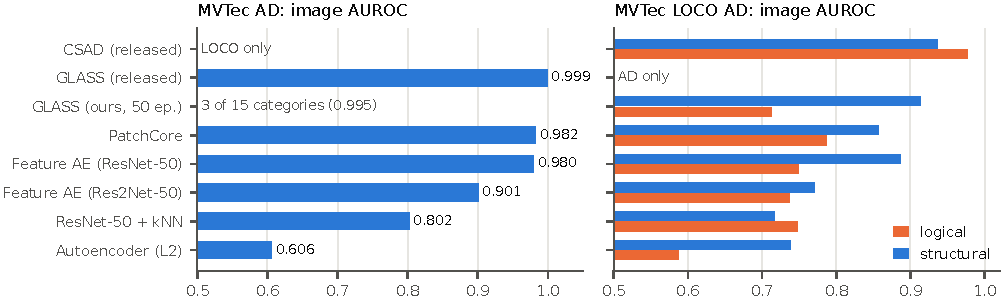
\includegraphics[width=\textwidth]{figures/auroc.pdf}
\caption{Image AUROC, mean over categories. Left: MVTec AD. Right: MVTec LOCO AD, split into logical (orange) and
structural (blue) anomalies. Released checkpoints were selected on the test set by their authors.}
\label{fig:auroc}
\end{figure*}

\begin{table}[t]
\caption{MVTec AD, mean over 15 categories. F1 uses the label-free threshold $\tau$; ms = per-image latency
(T4).}
\label{tab:ad}
\centering\footnotesize
\setlength{\tabcolsep}{3pt}
\resizebox{\columnwidth}{!}{%
\begin{tabular}{@{}lccccc@{}}
\toprule
Model & I-AUROC & P-AUROC & AUPRO & F1@$\tau$ & ms \\
\midrule
AE (L2) & 0.606\spm{}.001 & 0.751 & 0.509 & 0.152 & 7.9 \\
ResNet-50 + kNN & 0.802 & -- & -- & 0.515 & 7.7 \\
Feature AE (ResNet-50) & 0.980\spm{}.000 & 0.976 & 0.918 & \textbf{0.931} & 7.7 \\
Feature AE (Res2Net-50) & 0.901\spm{}.016 & 0.970 & 0.890 & 0.739 & 11.8 \\
PatchCore & 0.982 & 0.982 & 0.928 & 0.915 & 33.6 \\
GLASS, released & \textbf{0.999} & \textbf{0.993} & \textbf{0.969} & n/a & 31.9 \\
\bottomrule
\end{tabular}}
\end{table}

\begin{table}[t]
\caption{MVTec LOCO AD, mean over 5 categories (image AUROC).}
\label{tab:loco}
\centering\footnotesize
\setlength{\tabcolsep}{3.5pt}
\begin{tabular}{@{}lcccc@{}}
\toprule
Model & Logical & Structural & Mean & F1@$\tau$ \\
\midrule
AE (L2) & 0.587 & 0.738 & 0.662\spm{}.005 & 0.189 \\
ResNet-50 + kNN & 0.747 & 0.717 & 0.732 & 0.376 \\
Feature AE (ResNet-50) & 0.749 & 0.886 & 0.817\spm{}.002 & 0.592 \\
Feature AE (Res2Net-50) & 0.737 & 0.771 & 0.754\spm{}.033 & 0.382 \\
PatchCore & 0.786 & 0.857 & 0.822 & 0.490 \\
GLASS, ours (50 ep., last) & 0.713 & 0.913 & 0.813 & 0.530 \\
CSAD, released & \textbf{0.977} & \textbf{0.937} & \textbf{0.957} & \textbf{0.802} \\
\bottomrule
\end{tabular}
\end{table}

\subsection{Detection and localisation}
Fig.~\ref{fig:auroc} and Tables~\ref{tab:ad}--\ref{tab:loco} summarise the benchmark. Per-category results are in
Table~\ref{tab:percat} and the repository. On MVTec AD the embedding methods are close: PatchCore reaches 0.982
image AUROC. Roth et al.\ report 0.991 with a 224~px center crop that removes background~\cite{roth2022patchcore},
so our implementation is consistent. The feature autoencoder reaches 0.980 and the best F1 at the label-free
threshold (0.931). The released GLASS checkpoints lead on every metric. The plain autoencoder reconstructs many
defects and ranks near chance on several categories. ResNet-50 + kNN, which uses one global vector per image, misses
small defects (grid 0.334).

On LOCO, every model without explicit component reasoning stays below 0.79 logical AUROC, while CSAD reaches 0.977.
For structural anomalies the gap is smaller: GLASS trained by us reaches 0.913 against CSAD's 0.937. The ranking
supports the original report's design, which assigns a component-aware model to logical constraints.

\subsection{Audit of the original report}\label{sec:audit}
Table~\ref{tab:orig} compares the report with our runs. Where the report's numbers came from the team's own
models, ours agree in ranking and roughly in level. The autoencoder in particular reproduces the per-category
pattern (e.g.\ wood 0.94 vs 0.94, metal nut 0.30 vs 0.32). Five issues explain the remaining differences:
\begin{enumerate}
\item The ``Res2Net'' model used a ResNet-50 backbone. A real Res2Net-50 backbone does worse (0.901) and varies
more between seeds (grid 0.82$\pm$0.20).
\item Accuracy and F1 used thresholds tuned on test labels (F1-optimal on the test set). This explains
F1~$\approx$~0.97 in the report against 0.93 at a label-free threshold.
\item GLASS (0.999) and CSAD (0.957) match the authors' released checkpoints to four decimals. The team did not
train these models.
\item Two table rows are duplicated: PatchCore's \emph{pill} row equals the feature AE's, and the autoencoder's
\emph{zipper} F1 and runtime equal ResNet-50 + kNN's.
\item The runtime column mixes training time (AE, feature AE) with test time (kNN, PatchCore), without units or
hardware.
\end{enumerate}

\begin{table}[t]
\caption{Original report vs.\ this reproduction (mean image AUROC).}
\label{tab:orig}
\centering\footnotesize
\begin{tabular}{@{}lccc@{}}
\toprule
Model & Report & Ours & Note \\
\midrule
AE (L2) & 0.663 & 0.606 & no warm start \\
ResNet-50 + kNN & 0.739 & 0.802 & ImageNet normalisation \\
``Res2Net'' (feature AE) & 0.972 & 0.980 & ResNet-50 backbone \\
PatchCore & 0.959 & 0.982 & published method \\
GLASS & 0.999 & 0.999 & released ckpt. \\
CSAD (LOCO) & 0.957 & 0.957 & released ckpt. \\
\bottomrule
\end{tabular}
\end{table}

\subsection{Test-set checkpoint selection}\label{sec:selection}
The official GLASS script evaluates on the test set after every epoch and keeps the epoch with the highest image
plus pixel AUROC. CSAD's script does the same every 1,000 iterations. The released GLASS checkpoints record their
epoch: of 640 epochs, metal nut stops at 5, transistor at 52, capsule at 56, and wood at 637. To measure the effect,
we trained GLASS with the official code on all LOCO categories and on zipper, wood and transistor. We used 50
epochs instead of 640, since a T4 needs about 100~s per epoch. We logged the official test evaluation every five
epochs for analysis only. The last epoch is our reported model. On MVTec AD the two agree within 0.002
(0.995 vs 0.996). On LOCO, selection adds 0.015 mean AUROC and 0.046 logical AUROC, with +0.10 on pushpins
(Fig.~\ref{fig:selection}). Because the criterion mixes image and pixel scores, it also trades structural
performance away on pushpins and screw bag. Released scores of both methods are therefore upper bounds. The
optimism matters most on the harder LOCO benchmark.

\begin{figure}[t]
\centering
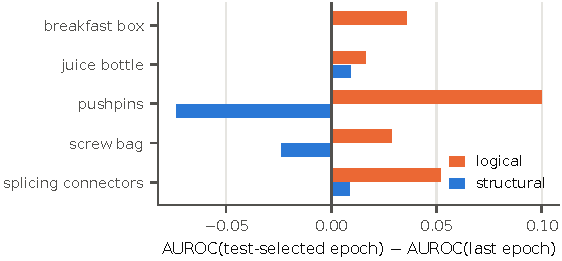
\includegraphics[width=\columnwidth]{figures/selection.pdf}
\caption{GLASS on LOCO: AUROC of the epoch the official script picks on the test set, minus that of the last
epoch.}
\label{fig:selection}
\end{figure}

\section{Deployment}\label{sec:platform}

\subsection{Platform}
AnoDe is a FastAPI service with a React interface that runs on a CPU (a Docker image is provided). The public demo
on Hugging Face Spaces is a static build: the deployed models were run once on every sample image, and the quality
control computations run in the browser, because free Spaces no longer host Docker containers. A user
picks a product, inspects images (upload, camera or a simulated line), sees a heatmap and segmentation per unit
(Fig.~\ref{fig:heatmaps}), and closes the batch. Batches feed a quality report. Users can add products of their own
from 10--100 images of good parts: PatchCore needs no training loop, so its memory bank is built on the server in
minutes, and 20\% of the images are held out to set $\tau$.

\begin{figure*}[t]
\centering
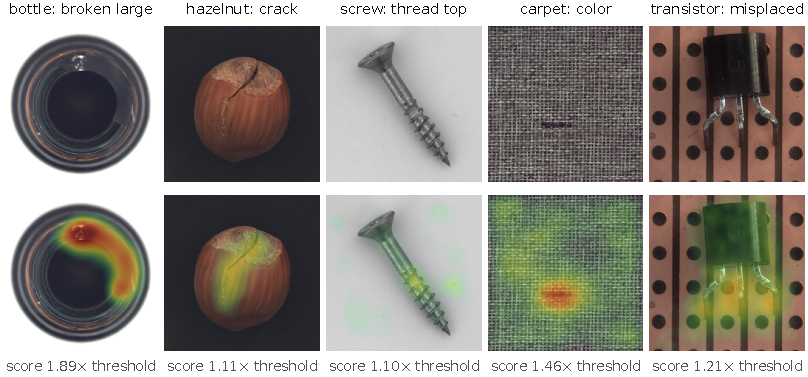
\includegraphics[width=\textwidth]{figures/heatmaps.pdf}
\caption{Deployed PatchCore on MVTec AD test images, as shown by the platform. Scores are given relative to the
product's threshold $\tau$; colour saturates at $2\tau$, and areas below $0.7\tau$ are left uncoloured.}
\label{fig:heatmaps}
\end{figure*}

\subsection{Which model can be deployed?}
A deployed detector needs a threshold, and a label-free threshold needs normal images the model has not seen.
Models trained on our split have them. The released GLASS checkpoints were trained on every normal training image,
and they score new normal images much higher than their own training images. With $\tau$ computed on images they
were trained on, they flag 33.5\% of good test parts. Their discriminator's natural 0.5 cut-off flags 31.7\%.
PatchCore flags 10.1\% and recalls 88.7\% of defects, and the feature AE flags 7.2\% and recalls 90.5\%
(Fig.~\ref{fig:calibration}). The platform therefore deploys PatchCore for MVTec AD products. For LOCO it deploys
the released CSAD checkpoints, which never train on the official validation split (1.8\% false alarms). CPU
latency on an Apple M1 is about 180~ms per image for PatchCore and 400~ms for CSAD.

\begin{figure}[t]
\centering
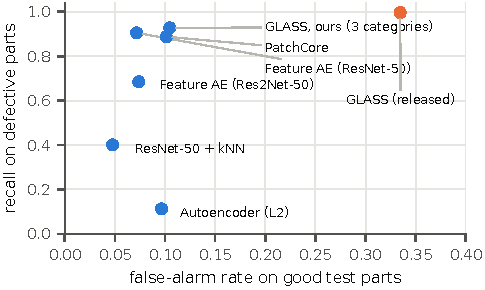
\includegraphics[width=\columnwidth]{figures/calibration.pdf}
\caption{MVTec AD at the label-free threshold $\tau$: false alarms on good parts vs.\ recall on defects. Released
GLASS uses $\tau$ from images it was trained on.}
\label{fig:calibration}
\end{figure}

\subsection{Robustness to image compression}
Cameras and browsers often deliver JPEG. On two good \emph{juice bottle} images, our CPU runtime reproduces the
official CSAD scores on the original PNGs (0.72 and $-0.22$ times $\tau$; official 0.51 and $-0.20$). Saving the
same images as JPEG at quality 90 moves them to 1.93 and 0.98 at full resolution, and to 3.17 and 1.36 at 512~px:
false alarms. Resizing to 512~px as PNG does not (0.49 and 0.19). PatchCore classified all 12 \emph{bottle} samples
correctly from JPEG. The platform stores samples as PNG and captures camera frames losslessly. Compression
robustness should be part of IAD evaluation.

\subsection{Statistical process control}
Each closed batch adds a point to a P-chart of the defective fraction. Its limits
$\bar p \pm 3\sqrt{\bar p(1-\bar p)/n_i}$ depend on the batch size $n_i$~\cite{montgomery2019sqc}. Process
capability is read from the continuous score $s/\tau$ against the upper specification limit USL $=1$:
\begin{equation}
C_{pk} = \frac{\text{USL} - \mu}{3\sigma}, \qquad C_{pk}^{\text{yield}} = \frac{\Phi^{-1}(1-p)}{3},
\end{equation}
where $p$ is the fraction above the USL. A batch that mixes good and defective parts has a bimodal score
distribution, which inflates $\sigma$. For 25 simulated batches drawn from real \emph{bottle} test scores
(Fig.~\ref{fig:spc}), the normal-theory index is 0.31, while the yield-based index, which is consistent with the
observed 3.2\% defect rate, is 0.62. The report shows both and flags the one out-of-control batch, which carries a
fourfold defect rate.

\begin{figure*}[t]
\centering
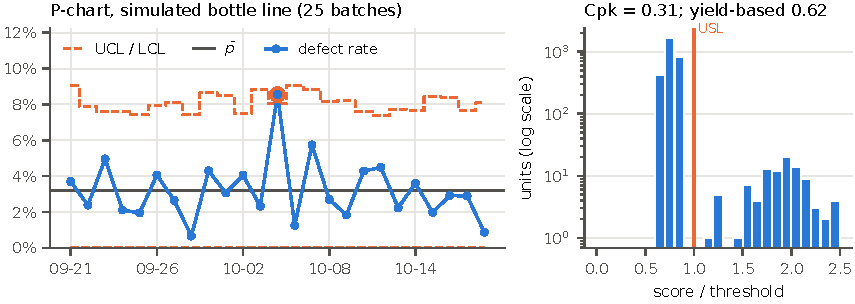
\includegraphics[width=\textwidth]{figures/spc.pdf}
\caption{Quality report for a simulated bottle line (2,987 units scored by the deployed PatchCore). Left: P-chart
with batch-size-dependent limits and one out-of-control batch. Right: score distribution (log scale) against
USL $=\tau$.}
\label{fig:spc}
\end{figure*}

\section{Limitations}
CSAD was not retrained (about 3~GPU-hours per category), so its scores carry the optimism quantified for GLASS.
GLASS was retrained with a short schedule (50 of 640 epochs) and one seed. Validation sets contain 6 (toothbrush)
to 69 (pushpins) normal images, so thresholds and false-alarm rates vary between categories. Latency was measured
on a T4 and on a laptop CPU, not on factory hardware. Finally, MVTec images are well lit and aligned, and real lines
will need their own normal images, which the custom-product workflow is designed for.

\section{Conclusion}
Rebuilding AnoDe from its report confirmed its main design: a strong local detector for surface defects and a
component-aware model for logical constraints. It also corrected the report's model description, threshold
practice and provenance of results. Two lessons apply beyond this project. Scores from checkpoints selected on the
test set should be reported as upper bounds, and the gap is largest on logical anomalies. A model is deployable only
if its threshold can be calibrated without test labels, which ranks PatchCore above a higher-scoring released GLASS
checkpoint in practice. Code, per-run results, the model bundle and the live platform are public.

\section*{Acknowledgment}
Experiments ran on free Kaggle GPUs. We thank the authors of GLASS and CSAD for releasing their code and
checkpoints, and MVTec Software GmbH for the datasets (CC BY-NC-SA 4.0).

\section*{Availability}
Code and results: \url{https://github.com/Peanut2Butter9/anode}. Platform:
\url{https://huggingface.co/spaces/Arzz/anode}. Models: \url{https://huggingface.co/Arzz/anode-models}.

\begin{thebibliography}{00}
\bibitem{liu2024survey} J. Liu, G. Xie, J. Wang, S. Li, C. Wang, F. Zheng, and Y. Jin, ``Deep industrial image anomaly detection: A survey,'' \emph{Machine Intelligence Research}, vol.~21, pp.~104--135, 2024.
\bibitem{bergmann2019mvtec} P. Bergmann, M. Fauser, D. Sattlegger, and C. Steger, ``MVTec AD -- A comprehensive real-world dataset for unsupervised anomaly detection,'' in \emph{Proc.\ CVPR}, 2019, pp.~9592--9600.
\bibitem{bergmann2021mvtec} P. Bergmann, K. Batzner, M. Fauser, D. Sattlegger, and C. Steger, ``The MVTec anomaly detection dataset: A comprehensive real-world dataset for unsupervised anomaly detection,'' \emph{Int.\ J.\ Comput.\ Vis.}, vol.~129, no.~4, pp.~1038--1059, 2021.
\bibitem{bergmann2022loco} P. Bergmann, K. Batzner, M. Fauser, D. Sattlegger, and C. Steger, ``Beyond dents and scratches: Logical constraints in unsupervised anomaly detection and localization,'' \emph{Int.\ J.\ Comput.\ Vis.}, vol.~130, pp.~947--969, 2022.
\bibitem{bergmann2019ssim} P. Bergmann, S. L\"owe, M. Fauser, D. Sattlegger, and C. Steger, ``Improving unsupervised defect segmentation by applying structural similarity to autoencoders,'' in \emph{Proc.\ VISAPP}, 2019, pp.~372--380.
\bibitem{cohen2020spade} N. Cohen and Y. Hoshen, ``Sub-image anomaly detection with deep pyramid correspondences,'' arXiv:2005.02357, 2020.
\bibitem{defard2021padim} T. Defard, A. Setkov, A. Loesch, and R. Audigier, ``PaDiM: A patch distribution modeling framework for anomaly detection and localization,'' in \emph{Proc.\ ICPR Workshops}, 2021, pp.~475--489.
\bibitem{roth2022patchcore} K. Roth, L. Pemula, J. Zepeda, B. Sch\"olkopf, T. Brox, and P. Gehler, ``Towards total recall in industrial anomaly detection,'' in \emph{Proc.\ CVPR}, 2022, pp.~14318--14328.
\bibitem{zavrtanik2021draem} V. Zavrtanik, M. Kristan, and D. Sko\v{c}aj, ``DRAEM -- A discriminatively trained reconstruction embedding for surface anomaly detection,'' in \emph{Proc.\ ICCV}, 2021, pp.~8330--8339.
\bibitem{liu2023simplenet} Z. Liu, Y. Zhou, Y. Xu, and Z. Wang, ``SimpleNet: A simple network for image anomaly detection and localization,'' in \emph{Proc.\ CVPR}, 2023, pp.~20402--20411.
\bibitem{chen2024glass} Q. Chen, H. Luo, C. Lv, and Z. Zhang, ``A unified anomaly synthesis strategy with gradient ascent for industrial anomaly detection and localization,'' in \emph{Proc.\ ECCV}, 2024.
\bibitem{hsieh2024csad} Y.-H. Hsieh and S.-H. Lai, ``CSAD: Unsupervised component segmentation for logical anomaly detection,'' in \emph{Proc.\ BMVC}, 2024.
\bibitem{batzner2024efficientad} K. Batzner, L. Heckler, and R. K\"onig, ``EfficientAD: Accurate visual anomaly detection at millisecond-level latencies,'' in \emph{Proc.\ WACV}, 2024, pp.~128--138.
\bibitem{he2016resnet} K. He, X. Zhang, S. Ren, and J. Sun, ``Deep residual learning for image recognition,'' in \emph{Proc.\ CVPR}, 2016, pp.~770--778.
\bibitem{zagoruyko2016wide} S. Zagoruyko and N. Komodakis, ``Wide residual networks,'' in \emph{Proc.\ BMVC}, 2016.
\bibitem{gao2021res2net} S.-H. Gao, M.-M. Cheng, K. Zhao, X.-Y. Zhang, M.-H. Yang, and P. Torr, ``Res2Net: A new multi-scale backbone architecture,'' \emph{IEEE Trans.\ Pattern Anal.\ Mach.\ Intell.}, vol.~43, no.~2, pp.~652--662, 2021.
\bibitem{montgomery2019sqc} D. C. Montgomery, \emph{Introduction to Statistical Quality Control}, 8th ed. Hoboken, NJ, USA: Wiley, 2019.
\end{thebibliography}

\appendix
\begin{table}[h]
\caption{Image AUROC per category. MVTec AD (top) and LOCO, mean of logical and structural (bottom). FAE = feature
autoencoder.}
\label{tab:percat}
\centering\scriptsize
\setlength{\tabcolsep}{2.4pt}
\begin{tabular}{@{}lccccccc@{}}
\toprule
Category & AE & kNN & FAE-R50 & FAE-R2N & PatchCore & GLASS$^\dagger$ & CSAD$^\dagger$ \\
\midrule
bottle & .727 & .974 & 1.00 & .997 & 1.00 & 1.00 & \\
cable & .488 & .799 & .983 & .917 & .993 & .998 & \\
capsule & .647 & .816 & .961 & .825 & .973 & .999 & \\
carpet & .371 & .703 & .981 & .979 & .988 & .998 & \\
grid & .878 & .334 & .982 & .820 & .987 & 1.00 & \\
hazelnut & .910 & .902 & 1.00 & .860 & 1.00 & 1.00 & \\
leather & .408 & .870 & 1.00 & 1.00 & 1.00 & 1.00 & \\
metal nut & .295 & .813 & 1.00 & .990 & .998 & 1.00 & \\
pill & .598 & .720 & .957 & .902 & .954 & .993 & \\
screw & .705 & .591 & .922 & .461 & .937 & 1.00 & \\
tile & .775 & .989 & 1.00 & .999 & 1.00 & 1.00 & \\
toothbrush & .567 & .803 & .961 & .919 & .928 & 1.00 & \\
transistor & .473 & .827 & .964 & .917 & .999 & .999 & \\
wood & .941 & .981 & .994 & .962 & .990 & .999 & \\
zipper & .301 & .910 & .991 & .959 & .983 & .999 & \\
\midrule
breakfast box & .623 & .803 & .848 & .825 & .818 & .832$^\ast$ & .928 \\
juice bottle & .661 & .868 & .955 & .937 & .956 & .961$^\ast$ & .957 \\
pushpins & .652 & .652 & .742 & .727 & .742 & .724$^\ast$ & .970 \\
screw bag & .700 & .581 & .709 & .651 & .708 & .755$^\ast$ & .971 \\
splicing conn. & .676 & .757 & .833 & .630 & .884 & .793$^\ast$ & .958 \\
\bottomrule
\multicolumn{8}{@{}l}{\scriptsize $^\dagger$released checkpoints; $^\ast$our training, 50 epochs, last epoch.}
\end{tabular}
\end{table}

\end{document}
